% 2017_zhejiang_q9_fig1: regular tetrahedron D-ABC, P midpoint AB, Q on BC (BQ:QC=2:1), R on CA (CR:RA=2:1).
% Base A-B-C; P-Q-R interior triangle dashed; D connected to all.
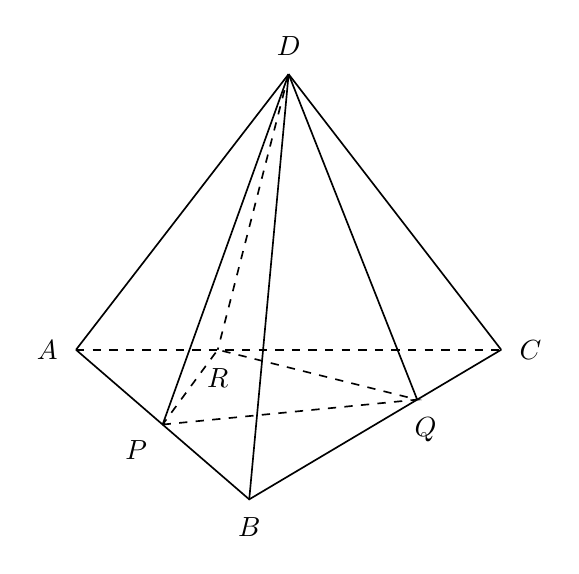
\begin{tikzpicture}[x=1cm,y=1cm,font=\normalsize,line width=.6pt]
\coordinate (D) at (3,6);
\coordinate (A) at (0.3,2.5);
\coordinate (B) at (2.5,0.6);
\coordinate (C) at (5.7,2.5);
\coordinate (P) at (1.4,1.55);
\coordinate (Q) at (4.6333333333,1.8666666667);
\coordinate (R) at (2.1000000000,2.5000000000);
% base perimeter solid except back AC dashed
\draw[solid,line width=.6pt] (A)--(P)--(B)--(Q)--(C);
\draw[dashed,line width=.6pt] (A)--(C);
% lateral edges
\draw[solid,line width=.6pt] (D)--(A);
\draw[solid,line width=.6pt] (D)--(P);
\draw[solid,line width=.6pt] (D)--(B);
\draw[solid,line width=.6pt] (D)--(Q);
\draw[solid,line width=.6pt] (D)--(C);
\draw[dashed,line width=.6pt] (D)--(R);
% interior triangle PQR dashed
\draw[dashed,line width=.6pt] (P)--(Q)--(R)--cycle;
\node[anchor=south,yshift=3pt] at (D) {$D$};
\node[anchor=east,xshift=-3pt] at (A) {$A$};
\node[anchor=north,yshift=-3pt] at (B) {$B$};
\node[anchor=west,xshift=3pt] at (C) {$C$};
\node[below left=2pt] at (P) {$P$};
\node[anchor=north,yshift=-3pt,xshift=3pt] at (Q) {$Q$};
\node[anchor=north,yshift=-3pt] at (R) {$R$};
\end{tikzpicture}
